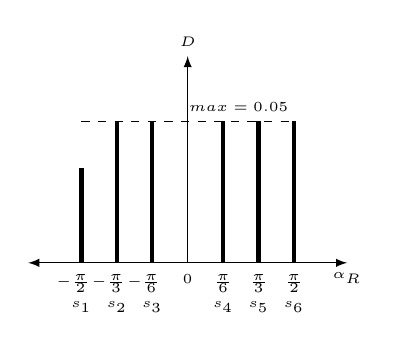
\begin{tikzpicture}[scale=0.75,font=\tiny]

% vector field histogram
\draw [-latex] (6,0) -- (8.7,0) node[at end, below]{$\alpha_R$};
\draw [-latex] (6,0) -- (3.3,0) ;
\draw [-latex] (6,0) -- (6,3.5) node[at start,below=0.8]{0} node[at end,above]{$D$};
\draw [dashed](4.2,2.4) -- (7.8,2.4) node[right=-20,above]{$max=0.05$};

\draw [ultra thick] (4.2,0) -- (4.2,1.6) node[at start,left=3,below]{$-\frac{\pi}{2}$} node[at start,below=10]{$s_1$};
\draw [ultra thick] (4.8,0) -- (4.8,2.4) node[at start,left=3,below]{$-\frac{\pi}{3}$} node[at start,below=10]{$s_2$};
\draw [ultra thick] (5.4,0) -- (5.4,2.4) node[at start,left=3,below]{$-\frac{\pi}{6}$} node[at start,below=10]{$s_3$};
\draw [ultra thick] (6.6,0) -- (6.6,2.4) node[at start,below]{$\frac{\pi}{6}$} node[at start,below=10]{$s_4$};
\draw [ultra thick] (7.2,0) -- (7.2,2.4) node[at start,below]{$\frac{\pi}{3}$} node[at start,below=10]{$s_5$};
\draw [ultra thick] (7.8,0) -- (7.8,2.4) node[at start,below]{$\frac{\pi}{2}$} node[at start,below=10]{$s_6$};

\end{tikzpicture}